\section{Flux Integral}

\subsection*{Overview}

Integrals over surfaces are difficult to visualize. There are scalar surface integrals which multiply the field by the surface area at each point on the surface, and there are vector surface integrals which measure the flux through that surface. These visualizations show the meaning of the surface tangent vectors \(T_u\) and \(T_v\). They also show the meaning of a flux integral of a vector field through a surface visually.

\subsection*{Implementation details}

This section is split into two visuals: one for scalar and one for vector fields. 

\textbf{Scalar surface integrals:} A 3D  plot is created using the scalar function of choice. The x partial and y partial are displayed using the vectors Then the vector $\langle 1, 0, \frac{\partial f}{\partial x} \rangle$ is depicted eminating from $\langle x, y, f(x, y) \rangle$. The cross product is produced by the vector $\langle \frac{\partial f}{\partial x}, \frac{\partial f}{\partial y}, 1 \rangle$. The x partial is green, the y is red, the cross product is blue. All of these are meshed using a mesh function and displayed as a single visual. \cite{flux8}

\textbf{Vector flux Integrals:} A 3D parametric function is displayed using the function \verb+param[u_, v_] =+ \verb+{Cos[u]*Sin[v],+ \verb+Sin[u]*Sin[v]+, \verb+Cos[v]}+ which of course in this example is the unit sphere. However, other parameterized surfaces can be chosen. The nice thing about using \verb+parametricPlot3D+ is level sets of u and v are also displayed on the surface. The u partials are the vectors \verb+{D[param[u, v][[1]], u],+ \verb+D[param[u, v][[2]], u],+ \verb+D[param[u, v][[3]], u]}+ which of course is the derivative of the parameterization based upon u and the v partial is calculated similarly except with respect to v. The u partial is red and the v is green. The normal is calculated by the the negative of the cross product of both partials in order to receive the outward facing normal. The vector field we chose for this demonstration was an interesting one: \verb+{Cos[u]^2/2, Sin[v]^3/2, Sin[u]*Cos[v]}+ which we overlaid and calculated only for the surface. Of course, any vector field may be chosen. The surface is semi-translucent to provide students the ability to look inside the parameterized surface. \cite{flux7}

\subsection*{Usage notes}

These models fully demonstrate all the parts needed to understand the components of these integrals. The surfaces, the partials, and the vector and scalar fields are all demonstrated in an easy to intuit manner. The models are incredibly customizable and will serve as practical means of demonstrating the concepts. 

These visualizations can be incorporated into lecture 31 Integrating over a Surface - Scalar valued functions and lecture 32 Surface Integrals (Flux).

\textbf{Scalar Surface Integrals:}
\begin{enumerate}
\item \verb+fieldF+ is the chosen scalar function.
\item \verb+xmin, xmax, ymin, ymax+ are the bounds of the domain.
\item \verb+xmid, ymid+ are the coordinates at which the partials and normal vector are calculated
\item All of these variables are free to edit and the program will accommodate to new models of choice
\end{enumerate}

\textbf{Vector-field Surface Integrals:}
\begin{enumerate}
\item \verb+umin, umax, vmin, vmax+ are the bounds of the parameters chosen. 
\item \verb+umid, vmid+ represent the coordinates at which the partials and the normal are calculated.
\item \verb+vectorincrementdensity+ is the increment in which the vectors are calculated along the surface. In simpler terms, a smaller number is a more detailed field and a bigger is a less detailed field. 
\item \verb+vectorfield+ is the the vector field that is chosen. 
\item All of these variables are free to edit and the program will accommodate to new models of choice
\end{enumerate}

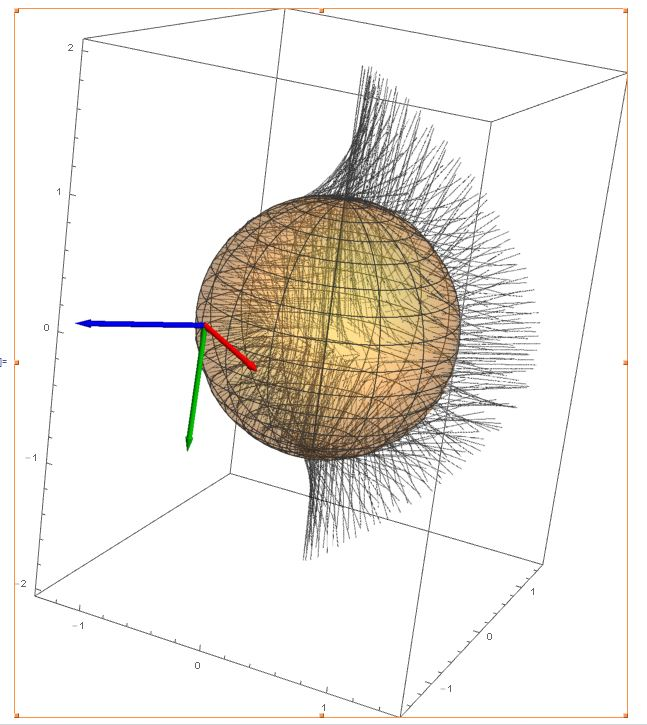
\includegraphics[height=10cm]{../exhibit/flux.jpg}

%%% Local Variables:
%%% mode: latex
%%% TeX-master: "main"
%%% End:
